%%%%%%%%%%%%%%%%%%%%%%%%%%%%%%%%%%%%%%%%%%%%%%%%%%%%%%%%%%%%%%%%%%%%%%%%%%%%%%%%%%%%%%%%%%%%%%%%%%%%%%%%%%%%%%%%%%%%%%%%%%%%%%%%%%%%%%%%%%%%%%%%%%%%%%
% 20141007 - Introduction to Operating Systems VO
%%%%%%%%%%%%%%%%%%%%%%%%%%%%%%%%%%%%%%%%%%%%%%%%%%%%%%%%%%%%%%%%%%%%%%%%%%%%%%%%%%%%%%%%%%%%%%%%%%%%%%%%%%%%%%%%%%%%%%%%%%%%%%%%%%%%%%%%%%%%%%%%%%%%%%

%fancyhdr
\lhead{IOS VO} 
\rhead{2014-10-07}

%%%%%%%%%%%%%%%%%%%%%%%%%%%%%%%%%%%%%%%%%%%%%%%%%%%%%%%%%%%%%%%%%%%%%%%%%%%%%%%%%%%%%%%%%%%%%%%%%%%%%%%%%%%%%%%%%%%%%%%%%%%%%%%%%%%%%%%%%%%%%%%%%%%%%%

\par{
	\noindent
	$n! = \text{factorial(n)} = \begin{cases}
		1 								&	\text{if n = 0}		\\
		\text{factorial}(n-1) \cdot n 	&	\text{otherwise}	\\
	\end{cases}
	\hspace{1cm}\Rightarrow O(n)$ \newline\newline
	$\underbrace{1024!}_{\text{just 4 digits but 1024 iterations/calls}} = O(2^d), d \ldots \text{number of digits}$ \newline\newline
	$n!$ is pseudo-polynomial!
}

\par{
	\noindent
	\texttt{1 0000 + 0 0001 = 1 0001} $\Rightarrow O(d)$ \newline
	Addition is much better because it has linear time complexity in the number of digits. If the computation is done numerically (the numbers are represented numerically), the time complexity is logarithmic in the size of digits: $O(log(d))$. \newline
	If we represent the number binary, the time complexity is doubly-exponential: $O\left(2^{2^d}\right)$.
}

\par{
	\noindent
	Considering the above recursion: There are at most $O(n)$ elements on the stack at any point of time (also in the worst case). Thus, this recursion has linear space complexity. \newline
	For some algorithm, e.g. sorting algorithms, the representation of the numbers has no effect because the numbers are only used in the comparison.
}

\par{
	\noindent\underline{Computability:}
	\par{
		\noindent
		\textbf{Alan Turing:} \newline
		There is no algorithm to decide whether an arbitrary program halts on a given input (1936). \textit{Halting problem}.
	}
	\par{
		\noindent
		\textbf{Rice:} \newline
		Generalization to any non-trivial property of partial functions (programs that may or may not terminate) computed by arbitrary programs. A compiler can not analyze a program for an arbitrary property.
	}
	\par{
		\noindent
		\textbf{Church:} \newline
		1 month earlier than Turing using $\lambda$-calculus.
	}
}

\par{
	\noindent\underline{Proof sketch:} \newline
	\indent total function: defined on our inputs \newline
	\indent partial function: will not terminate for inputs for which it is not defined
	\begin{enumerate}
		\item{
			$h(i, x) = \begin{cases}
				1 	&	\text{program } i \text{ halts on } x	\\
				0 	&	\text{otherwise}					\\
			\end{cases}$ \newline
			$h(i, x)$ is a total, computable function.
		}
		\item{Let $f$ be any total, computable function with two arguments (in fact it may even be $h(i, x)$).}
		\item{
			$g(i) = \begin{cases}
				0 					&	\text{if } f(i, i) = 0 	\\
				\text{undefined}	&	\text{otherwise}
			\end{cases}$ \newline\newline
			Equivalent program code: \newline
			\texttt{   if(f(i, i) == 0) return 0;} \newline
			\texttt{else while(true) \{\};} \newline\newline
			$g(i)$ is a partial, computable function.
		}
		\item{$g(i)$ may be partial but is computable by a program $e$ (as described in the step before).}
		\item{
			If $f(e, e) = 0$: $g(e) = 0$ by definition $\Rightarrow h(e, e) = 1$. \newline
			If $f(e, e) \not= 0$: $g(e) = \text{undefined}$ (does not terminate) $\Rightarrow h(e, e) = 0$. \newline
			$\Rightarrow f$ is always different from $h \Rightarrow h$ can not be programmed.
		}
	\end{enumerate}
	This proof technique is called \textit{Diagonalization} and was introduced by Cantor in 1891.
}

\par{
	\noindent
	Given 2 infinite sets: which one is bigger (cardinality)? \newline
	E.g. $\mathbb{N}$ vs. $P(\mathbb{N})$: $\mathbb{N} < P(\mathbb{N})$ (strictly bigger!)
}

\par{
	\noindent
	$\mathbb{N}$: There are enough natural numbers to encode any program you can ever think of. \newline
}

\par{
	\noindent\underline{Another view on the halting problem:}
	\begin{figure}[!htb]
		\centering
		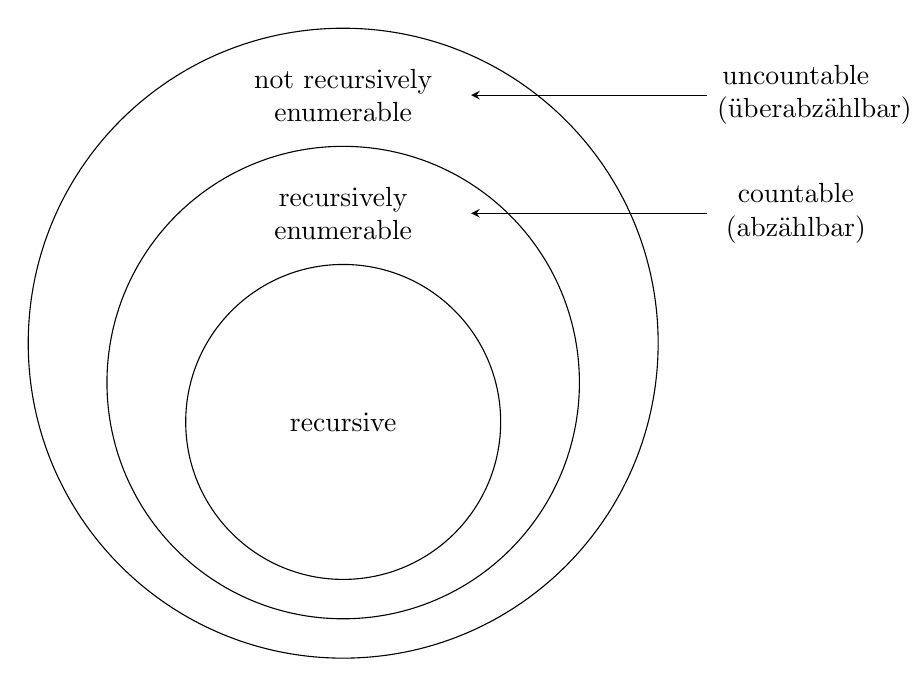
\begin{tikzpicture}
			\draw (0, 1) circle (4cm);
			\draw (0, 0.5) circle (3cm);
			\draw (0, 0) circle (2cm);

			\node[text width = 3cm, text centered] (nre_t) at (0, 4.15) {not recursively enumerable};
			\node[text width = 3cm, text centered] (re_t) at (0, 2.65) {recursively enumerable};
			\node[text width = 3cm, text centered] (r_t) at (0, 0) {recursive};

			\draw[<-, >=stealth] (nre_t.east) -- ++(3, 0) node[right, text width = 2cm, text centered] {uncountable ({\"u}berabz{\"a}hlbar)};
			\draw[<-, >=stealth] (re_t.east) -- ++(3, 0) node[right, text width = 2cm, text centered] {countable (abz{\"a}hlbar)};
		\end{tikzpicture}
		\caption{The halting problem in terms of languages.}
		\label{fig:diffviewhaltingprob}
	\end{figure}
	\begin{itemize}
		\item{
			Recursive: \newline
			A language (a set of strings) is recursive if it is accepted by a Turing machine which always terminates/halts.
		}
		\item{
			Recursively enumerable (r. e.): \newline
			A language is recursively enumerable if it is accepted by a Turing machine which may terminate/halt on a string not in the language.
			$\{(i, x) | \text{program } i \text{ halts on } x\}$
		}
		\item{
			Not recursively enumerable (n. r. e.): \newline
			Is actually \underline{not} a superset of the r. e. set but n. r. e. $\cup$ r. e. results in the set of all reachable programs. This set is uncountable.
			$\{(i, x) | \text{program } i \text{ does not halt on } x\}$
		}
	\end{itemize}
}

\par{
	\noindent
	\begin{figure}[!htb]
		\centering
		\begin{tikzpicture}
			\node (algorithm_t) at (2, 2) {algorithm};
			\node[below left = 1 and 0.25 of algorithm_t] (cost_t) {cost};
			\node[below right = 1 and 0.25 of algorithm_t] (computability_t) {computability};
			\node[right = 1 of algorithm_t] (problem_t) {problem};

			\draw[->, >=stealth] (algorithm_t.south west) -- (cost_t.north);
			\draw[->, >=stealth] (algorithm_t.south east) -- (computability_t.north);
			\draw[->, >=stealth] (algorithm_t.east) -- (problem_t.west);
			\draw[->, >=stealth] (problem_t.east) -- ++(1, 0) node[right, text width = 4cm] (np-completeness) {NP-completeness: problem is hard of NP ($\in$NP) (can be solved by a deterministic Turing machine in polynomial time) $\rightarrow$ upper bound statement};
			\node[right = 0 of np-completeness, text width = 4cm] (np-hardness) {NP-hardness: problem is in the category of NP-complete problems $\rightarrow$ lower bound statement};
		\end{tikzpicture}
		\caption{NP-completeness \& NP-hardness}
		\label{fig:npcompletenesshardness}
	\end{figure}
}

\par{
	\noindent
	In full generality, a compiler cannot choose whether a code is dead or not \newline
	$\Rightarrow$ NP-hard. \newline
	In some trivial cases, the compiler can actually recognize dead code.
}

\par{
	\noindent\underline{Syntax \& Semantics:}
	\par{
		\noindent
		Syntax: Parser, Syntax analysis, \ldots \newline
		Semantics: Code generator, semantics definition, \ldots \newline
		In combination: compiler
	}
	\par{
		\noindent Syntax:
		\parskip0pt\begin{enumerate}
			\item{What is correct syntax? Specification}
			\item{Parser}
		\end{enumerate}
	}
	\par{
		\noindent
		Example: \texttt{1 + (2 + y) * z} \newline\newline
		\underline{Grammar:}
		\par{
			\noindent
			\begin{center}
				\begin{tabular}{|l|l|}	
					\hline
					Symbol 									&	Description		\tabularnewline
					\hline
					\texttt{<string> (e.g. expression)}		&	non-terminal	\tabularnewline
					\texttt{"<string>" (e.g. "a")}			&	terminal 		\tabularnewline
					\texttt{[<symbol>] (e.g. ["-"])}		&	optionality		\tabularnewline
					\texttt{\{<symbol>\} (e.g. \{digit\})}	&	repetition		\tabularnewline
					\texttt{|}								&	OR 				\tabularnewline
					\hline
				\end{tabular}
			\end{center}
		}
		\noindent Parser: context-free $\rightarrow$ counts symbols (e.g. matching parentheses); Recursive-decent parser
		\parskip0pt\begin{itemize}
			\item[]{\texttt{expression := ["-"] term \{("+" | "-") term\}.}}
			\item[]{\texttt{term := factor \{("*" | "/") factor\}.}}
			\item[]{\texttt{factor := identifier | integer | "(" expression ")".}}
		\end{itemize}
		Scanner (FSM): reads character-wise and decides; regular $\rightarrow$ if you can transform this into a single equation
		\parskip0pt\begin{itemize}
			\item[]{\texttt{identifier := letter \{letter | digit\}.}}
			\item[]{\texttt{letter := "a" | "b" | \ldots | "z" | "A" | "B" | \ldots | "Z".}}
			\item[]{\texttt{digit := "0" | "1" | \ldots | "9".}}
			\item[]{\texttt{integer := digit \{digit\}.}}
		\end{itemize}
	}
	\par{
		\noindent\underline{Implementation of \texttt{expression()}:}
		\par{
			\noindent
			\texttt{expression() \{} \newline
			\indent\texttt{if(symbol == MINUS)} \newline
			\indent\indent\texttt{getSymbol(); // next symbol} \newline
			\indent\texttt{term();} \newline
			\indent\texttt{while((symbol == PLUS) || (symbol == MINUS)) \{} \newline
			\indent\indent\texttt{getSymbol();} \newline
			\indent\indent\texttt{term();} \newline
			\indent\texttt{\}} \newline
			\texttt{\}}
		}
		\par{\noindent So far no semantics!}
	}
}
